\chapter{项目特色}

\subsection{商家页面及部分功能的设计}
我们通过对用户身份的标记,允许部分普通用户申请成为商家用户,成为商家用户之后,个人主页将会显示店铺管理入口,在店铺主页提供对店铺的管理项.

\begin{figure}[h]
    \centering
        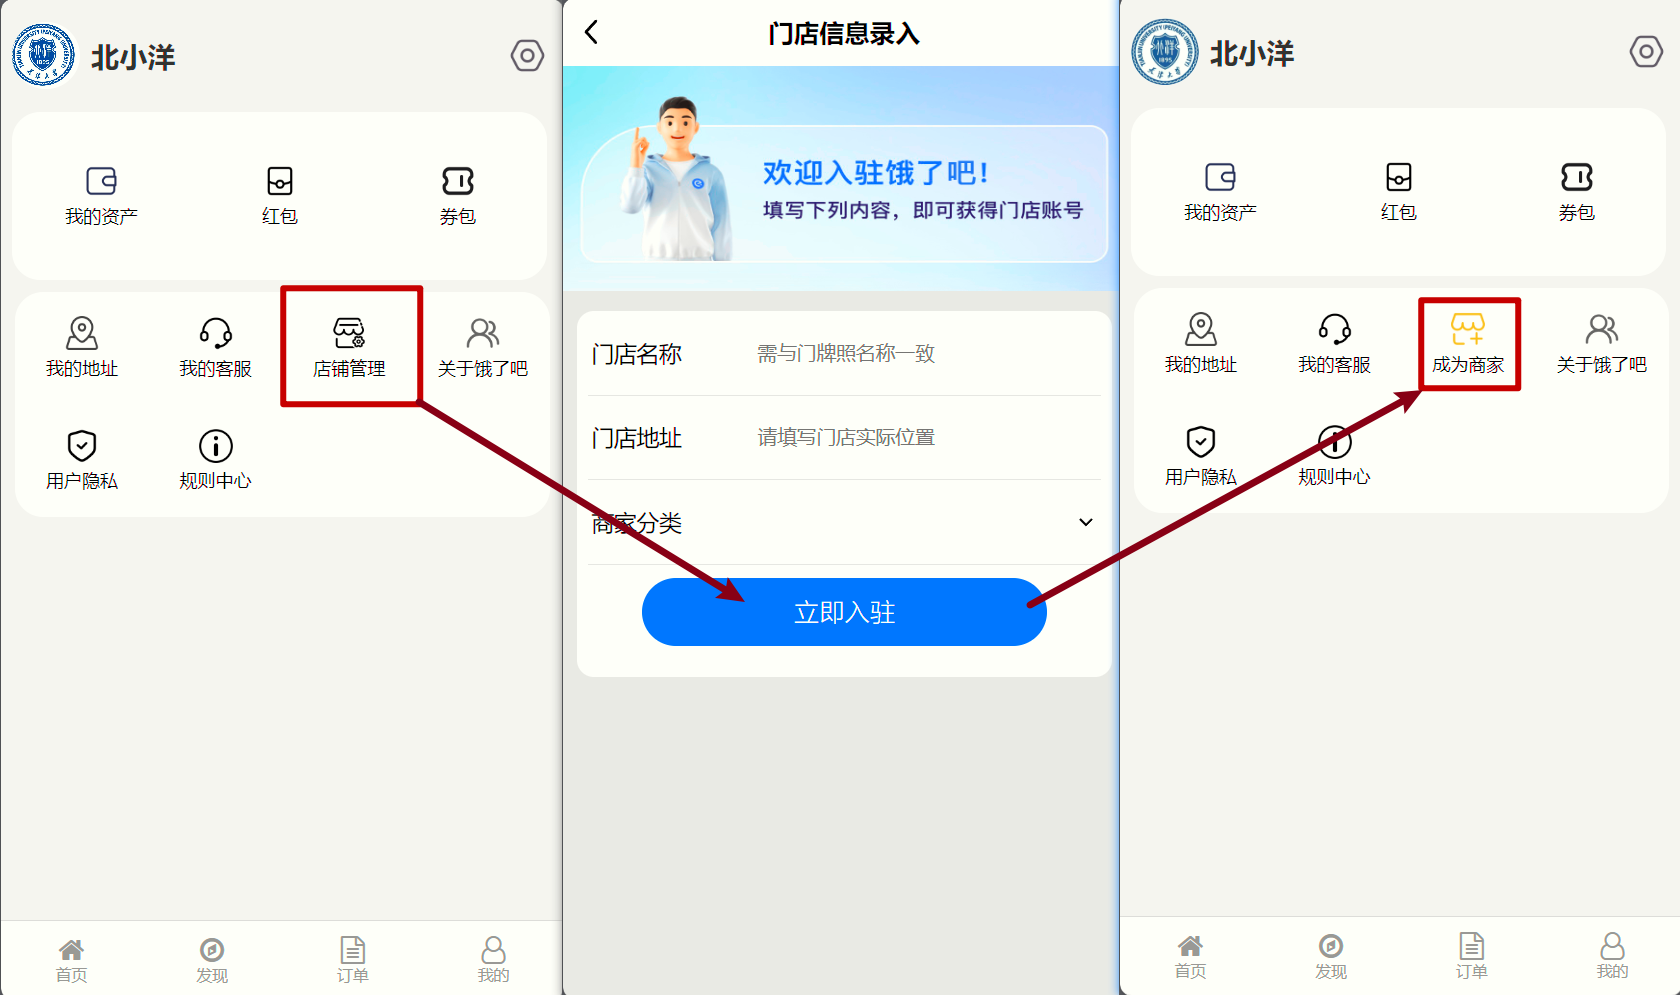
\includegraphics[width=0.75\linewidth]{uiFigs/成为商家.png}
    \caption{商家注册示意图}
    \label{fig:sjzc}
\end{figure}




\subsection{重构软件提示框}
饿了吧V1.0面对用户的提示框使用的浏览器默认的提示框,该提示框对用户显示操作不友好,于是我们重新设计提示函数,添加公共组件,设计出用户友好的提示显示框.
\begin{figure}[H]
    \centering
        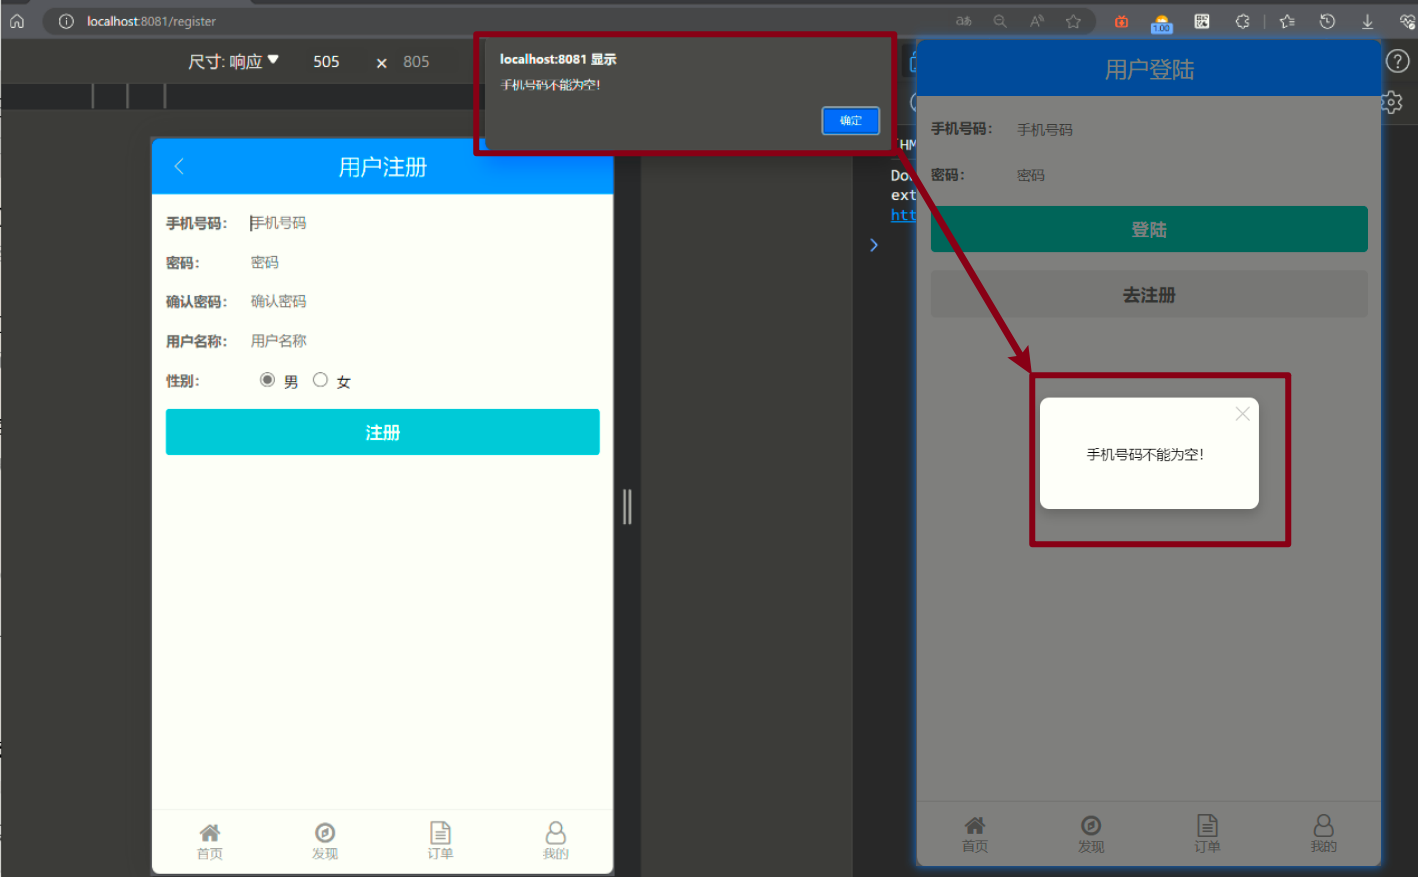
\includegraphics[width=0.75\linewidth]{uiFigs/弹窗风格.png}
    \caption{弹窗风格设计图}
    \label{fig:tcfg}
\end{figure}

\subsection{巧妙解决历史订单修改问题}\label{con:6.03}
对订单中涉及的商品名称、价格等信息进行修改时,会引起历史订单信息的修改,最普通的做法是新建一个历史订单的表,我们小组经过商议决定对数据库结构进行适当修改,在food和deliveraddress表添加delTag字段实现"假删除"与"假更新",从而保证历史订单读取的是历史数据,从而巧妙地解决了这个问题,同时减少了代码地修改量,对数据库结构的修改也有利于后续功能的实现.
\subsection{人机验证功能的添加}
前后端实现了人机验证功能,即在用户选择某一个商品时,商品数量超过特定数量时会弹出人机验证弹窗,输入正确的验证码后即可继续添加商品数量,否则拒绝请求.详细实现参考项目设计介绍\ref{con:rjyz}

